\documentclass[tikz,border=3pt]{standalone}
\usepackage[utf8]{inputenc}
\usepackage[T1]{fontenc}
\usepackage{lmodern}
\renewcommand{\familydefault}{\sfdefault}
\usepackage{sansmath}\sansmath
\usepackage{chemfig}
\usepackage{pgfplots}\pgfplotsset{compat=1.18,/pgf/number format/use comma,/pgf/number format/1000 sep={.}}
\usetikzlibrary{arrows.meta,calc,positioning,decorations.pathmorphing,patterns}
% paleta del sitio
\definecolor{nar}{HTML}{E8680C}\definecolor{narc}{HTML}{FFB35C}\definecolor{hielo}{HTML}{FFF3E8}
\definecolor{tinta}{HTML}{1D1D1F}\definecolor{gris}{HTML}{6E6E73}\definecolor{lila}{HTML}{7C5CF0}
\definecolor{azul}{HTML}{2F6FD6}\definecolor{menta}{HTML}{17A673}\definecolor{coral}{HTML}{E8342A}
\begin{document}
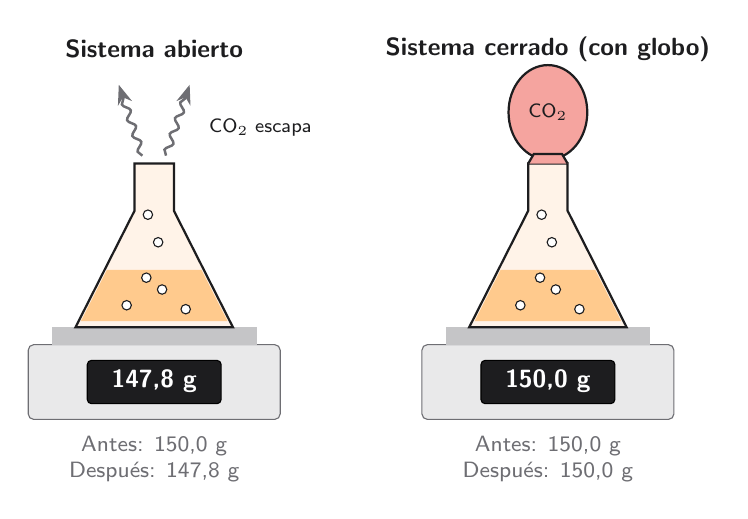
\begin{tikzpicture}
\node[font=\sffamily\small\bfseries,text=tinta] at (0,3.75) {Sistema abierto};
\draw[fill=gris!15,draw=gris,rounded corners=2pt] (-1.6,-0.95) rectangle (1.6,0);
\fill[gris!40] (-1.3,0) rectangle (1.3,0.22);
\draw[fill=tinta,rounded corners=1.5pt] (-0.85,-0.75) rectangle (0.85,-0.2);
\node[text=white,font=\sffamily\small\bfseries] at (0,-0.47) {147,8 g};
\draw[fill=hielo,draw=tinta,line width=0.8pt] (-1,0.22) -- (-0.25,1.7) -- (-0.25,2.3) -- (0.25,2.3) -- (0.25,1.7) -- (1,0.22) -- cycle;
\fill[narc!70] (-0.93,0.3) -- (-0.6,0.95) -- (0.6,0.95) -- (0.93,0.3) -- cycle;
\foreach \bx/\by in {-0.35/0.5, 0.1/0.7, 0.4/0.45, -0.1/0.85, 0.05/1.3, -0.08/1.65} \draw[tinta,fill=white] (0+\bx,\by) circle (0.06);
\node[font=\sffamily\footnotesize,text=gris,align=center] at (0,-1.45) {Antes: 150,0 g\\ Después: 147,8 g};

\draw[-{Stealth},gris,line width=0.9pt,decorate,decoration={snake,amplitude=1.2pt,segment length=6pt,post length=3pt}] (-0.15,2.4) -- (-0.45,3.3);
\draw[-{Stealth},gris,line width=0.9pt,decorate,decoration={snake,amplitude=1.2pt,segment length=6pt,post length=3pt}] (0.15,2.4) -- (0.45,3.3);
\node[font=\sffamily\scriptsize,text=tinta] at (1.35,2.75) {CO$_2$ escapa};

\node[font=\sffamily\small\bfseries,text=tinta] at (5,3.75) {Sistema cerrado (con globo)};
\draw[fill=gris!15,draw=gris,rounded corners=2pt] (3.4,-0.95) rectangle (6.6,0);
\fill[gris!40] (3.7,0) rectangle (6.3,0.22);
\draw[fill=tinta,rounded corners=1.5pt] (4.15,-0.75) rectangle (5.85,-0.2);
\node[text=white,font=\sffamily\small\bfseries] at (5,-0.47) {150,0 g};
\draw[fill=hielo,draw=tinta,line width=0.8pt] (4,0.22) -- (4.75,1.7) -- (4.75,2.3) -- (5.25,2.3) -- (5.25,1.7) -- (6,0.22) -- cycle;
\fill[narc!70] (4.07,0.3) -- (4.4,0.95) -- (5.6,0.95) -- (5.93,0.3) -- cycle;
\foreach \bx/\by in {-0.35/0.5, 0.1/0.7, 0.4/0.45, -0.1/0.85, 0.05/1.3, -0.08/1.65} \draw[tinta,fill=white] (5+\bx,\by) circle (0.06);
\node[font=\sffamily\footnotesize,text=gris,align=center] at (5,-1.45) {Antes: 150,0 g\\ Después: 150,0 g};

\draw[fill=coral!45,draw=tinta,line width=0.8pt] (5,2.95) ellipse (0.5 and 0.6);
\draw[fill=coral!45,draw=tinta,line width=0.8pt] (4.75,2.3) -- (4.82,2.42) -- (5.18,2.42) -- (5.25,2.3);
\node[font=\sffamily\scriptsize,text=tinta] at (5,2.95) {CO$_2$};
\end{tikzpicture}
\end{document}
